\documentclass{sigchi}

% Load basic packages
\usepackage{balance}       % to better equalize the last page
\usepackage{graphics}      % for EPS, load graphicx instead
\usepackage[T1]{fontenc}   % for umlauts and other diaeresis
\usepackage{txfonts}
\usepackage{mathptmx}
\usepackage[pdflang={en-US},pdftex]{hyperref}
\usepackage{color}
\usepackage{booktabs}
\usepackage{textcomp}

% Some optional stuff you might like/need.
\usepackage{microtype}        % Improved Tracking and Kerning
% \usepackage[all]{hypcap}    % Fixes bug in hyperref caption linking
\usepackage{ccicons}          % Cite your images correctly!
% \usepackage[utf8]{inputenc} % for a UTF8 editor only

% Paper metadata (use plain text, for PDF inclusion and later
% re-using, if desired).  Use \emtpyauthor when submitting for review
% so you remain anonymous.
\def\plaintitle{Physical Effort and Expressivity in\\ Electronic Musical Instruments}
\def\plainauthor{Tom Gurion}
\def\plainkeywords{effort; expression; electronic music instruments}

% llt: Define a global style for URLs, rather that the default one
\makeatletter
\def\url@leostyle{%
  \@ifundefined{selectfont}{
    \def\UrlFont{\sf}
  }{
    \def\UrlFont{\small\bf\ttfamily}
  }}
\makeatother
\urlstyle{leo}

% To make various LaTeX processors do the right thing with page size.
\def\pprw{8.5in}
\def\pprh{11in}
\special{papersize=\pprw,\pprh}
\setlength{\paperwidth}{\pprw}
\setlength{\paperheight}{\pprh}
\setlength{\pdfpagewidth}{\pprw}
\setlength{\pdfpageheight}{\pprh}

% Make sure hyperref comes last of your loaded packages, to give it a
% fighting chance of not being over-written, since its job is to
% redefine many LaTeX commands.
\definecolor{linkColor}{RGB}{6,125,233}
\hypersetup{%
  pdftitle={\plaintitle},
  pdfauthor={\plainauthor},
  pdfkeywords={\plainkeywords},
  pdfdisplaydoctitle=true, % For Accessibility
  bookmarksnumbered,
  pdfstartview={FitH},
  colorlinks,
  citecolor=black,
  filecolor=black,
  linkcolor=black,
  urlcolor=linkColor,
  breaklinks=true,
  hypertexnames=false
}

% create a shortcut to typeset table headings
% \newcommand\tabhead[1]{\small\textbf{#1}}

% End of preamble. Here it comes the document.
\begin{document}

\title{\plaintitle}

\numberofauthors{1}
\author{%
  \alignauthor{Tom Gurion\\
    \affaddr{Media and Arts Technology}\\
    \affaddr{Queen Mary University of London}\\
    \email{t.gurion@qmul.ac.uk}}\\
}

\maketitle

% TODO abstract
\begin{abstract}
  Lorem ipsum dolor sit amet, consectetur adipisicing elit, sed do eiusmod tempor incididunt ut labore et dolore magna aliqua. Ut enim ad minim veniam, quis nostrud exercitation ullamco laboris nisi ut aliquip ex ea commodo consequat. Duis aute irure dolor in reprehenderit in voluptate velit esse cillum dolore eu fugiat nulla pariatur. Excepteur sint occaecat cupidatat non proident, sunt in culpa qui officia deserunt mollit anim id est laborum.
An initial study explore this questions and highlight relationship
TODO performer point of view.
TODO Initial study.
TODO proposes framework to explore performer and listeners points of view.
In addition, it explores the effect of the performer's physical effort on the audience perception and appreciation of the performance.
These questions are assessed in controlled experiment, evaluating perceived expressivity from the point of view of the performer and the listener alike.

\end{abstract}

\keywords{\plainkeywords}

\section{Introduction}

During the 20th century electronic music interfaces evolved from mimicking acoustic instrument, like the piano keyboard or drums, to use novel techniques to control sound \cite{Paradiso1997}.
Examples include tabletop interfaces \cite{Jorda2007}, wearables \cite{Mitchell2012}, and biofeedback devices like EEG helmets \cite{Miranda2005}.
In parallel to these changes, research and design of new instruments started to separate the physical interface from the audio generation unit \cite{Cook2004}.
This model therefor describes most instruments by means of control unit, audio generation unit, and the mapping that tie them together \cite{Drummond2009}.
As a result, new interfaces often break the apparent relationship between how the instrument is played and the resulted sound \cite{DEscrivan2006}.

One significant difference between traditional and electronic music performances is that physical effort is usually involve in the former, but can be totally absent from the later.
This problem is often attributed to the ideal of "effortless interaction" that computers propose \cite{Ryan1992}.
Whereas this ideal is perfectly viable for designing software to browse the internet or write documents, it is less appropriate for most creative processes.
Another issue is that computers and by extension several electronic music interfaces prevent embodied interactions by their very nature \cite{Armstrong2006}.

Apart from the expressivity of the performer, the ability of the listener to understand the performance might also depend on the relationship between visible effort and the resulted sound \cite{Verdonk2015}.
This idea is discussed thoroughly in the context of live laptop music \cite{Schloss2003}.
In these type of performances, more often than not, the performer stares on the laptop screen, motionless, while operating the music software.
The relationship between cause and effect in these performances lacks any visual cues.
On extreme cases, a listener might question the "liveness" of a performance altogether when unable to tell the difference between live and pre-composed playback.
Besides, visible effort is an important expressive tool in many musical contexts \cite{Schloss2003}.
Consider, for example, a trumpet player and his out-curved veins in the neck while reaching a high note, or a drummer, sweating during intense performance.
These visible expressions usually have significant effect on the audience appreciation of the performance.
Most of the research in the field, however, doesn't confront the theoretical hypotheses using rigorous experiments.
One exceptional experiment based study confirms this hypothesis by showing that when listeners fail to build mental model of how an electronic instrument work they start to rely on facial expression and visible cues to assess errors in performance \cite{Fyans2010}.
Another experiment based study argues against the hypothesis by showing that experienced listeners do able to perceive what the performer is doing from the audio alone \cite{Bown2014}.
Other researchers approach this issue by suggesting the re-education the audience to appreciate ``aural'' performativity instead of visual spectacles \cite{Stuart2003}.
They support their arguments by examples from traditions that accepted the lack of visual cues in musical performances, like tape music concerts, and different variances of sound installations.

Recently, researchers suggested frameworks to assess the expressive possibilities of new interfaces for music performance \cite{Poepel2005}.
In their model, performers communicate emotions by ``coding'' them with a set of musical properties.
Specifically, they mention tempo, sound level, timing, intonation, articulation, timbre, vibrato, tone attacks, tone decays and pauses.
The listeners, on the other hand, ``decode'' these properties to understand the performer expressive intention.
This model for understanding expression in performance was validated in controlled experiment \cite{Gabrielsson1996}.
Now, new interfaces for music performance should provide the means to control these properties to allow the performer to convey emotion.
But controllability is probably not enough.
New interfaces should consider the interface ``efficiency'' - the ratio between the complexity of the resulted sound and the complexity of the controller input \cite{Jorda2004}.
In addition, the ability to master the instrument, questions of controllability versus randomness, and physical feedback should all be taken into account \cite{Dobrian2006}.

\section{Initial study}

The current study examines to what extent physical effort can enhance expressivity in playing electronic instruments.
To address this question I use the Schleikess interface, a digital controller for interactive performance that requires physical effort and large body movements from the performer.
Figure \ref{fig:schleikess} shows a schematic diagram of the interface.
It is composed of two elastic bands, each of them is connected with one side, through a load sensor, to a belt loop of the performer.
The load sensor measures the tension of the elastic band as it stretches and transmit this information to the computer to translate it to sound.
The performer holds the other side of the elastic bands and can stretch them to play.

\begin{figure}
  \centering
  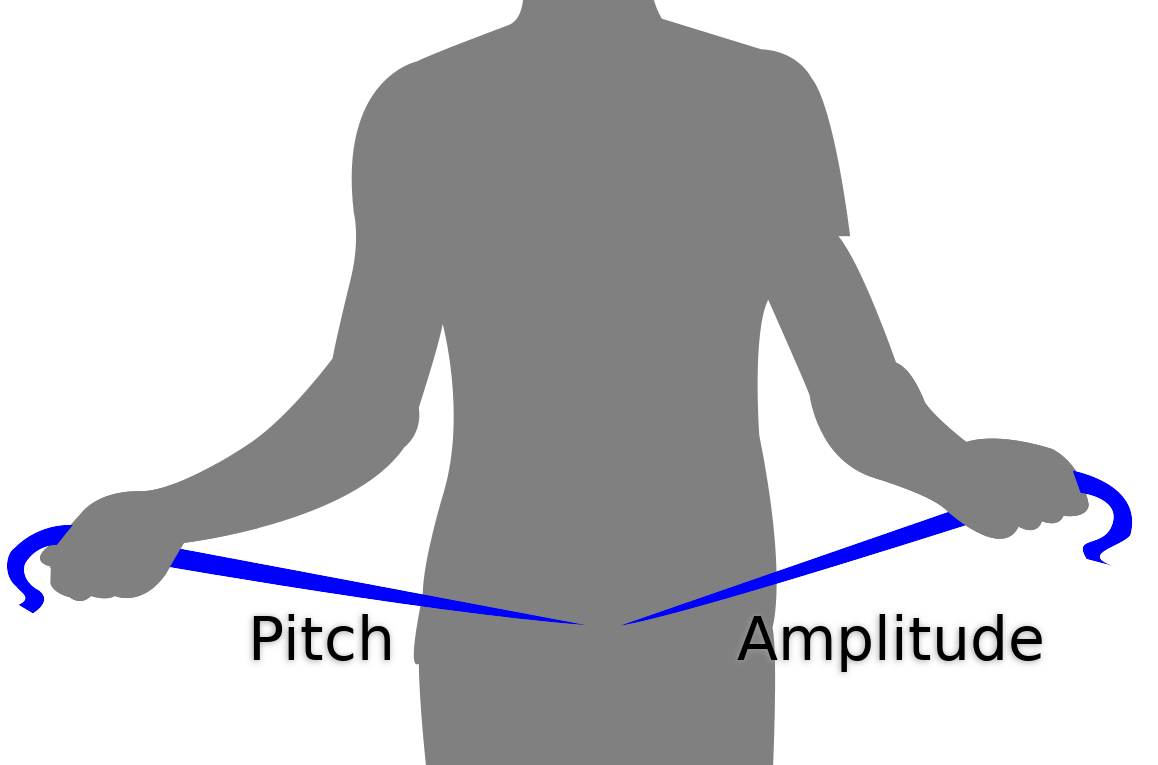
\includegraphics[width=0.9\columnwidth]{figures/schleikess}
  \caption{A diagram of the Schleikess interface. In blue are the two elastic bands. Stretching the left raises the pitch and stretching the right raises the amplitude of a sawtooth tone generator.}~\label{fig:schleikess}
\end{figure}

Although this controller can be used for different creative purposes, in the context of this study one elastic band controls the pitch and the other controls the amplitude of a sawtooth tone generator.
This type of interaction resembles the design of the theremin \cite{Theremin1996}.
Choosing this type of design provide several advantages for assessing the question of expressivity and physical effort.
First, as noted in \cite{Fyans2010}, it proposes a simple relationship between performer gesture and sound.
Considering that the participants in the study had no former familiarity with the interface, this by itself allow them to understand the interactive behavior good enough to provide valuable feedback.
Second, the added effort required by the Schleikess doesn't complicate the understanding of the instrument but provide the opportunity to test the questions of physical effort and expressivity directly.

\subsection{Methods}

Eight participants were invited to play with the Schleikess based synthesizer and discuss their subjective experience.
Apart from the physical interface, figure \ref{fig:pd-interface} shows the interface on the computer screen that was exposed to the participants.
The interface presents three sliders.
The first two control the sensitivity of each elastic band to force.
So, when the sensitivity is set to low value, a major physical effort is needed to raise the pitch or amplitude, but when the sensitivity is set to high value even minor changes affect the output significantly.
The last slider controls the overall volume of the instrument and allows the participant to set it to a comfortable hearing level.

\begin{figure}
  \centering
  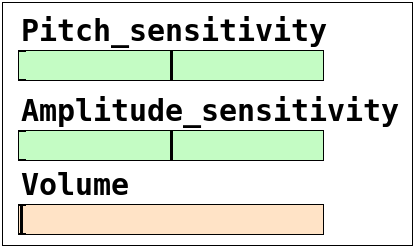
\includegraphics[width=0.9\columnwidth]{figures/pd_interface}
  \caption{The Schleikess graphical interface. Three sliders control the sensitivity of the pitch band to force, the sensitivity of the amplitude band to force, and the overall volume of the instrument.}~\label{fig:pd-interface}
\end{figure}

First, I explained to the participants that stretching the elastic bands controls the instrument.
The relationship between stretching the bands and the resulted sound was not explained.
Than, the participants were asked to play the instrument, listening to it through headphones, until they understand the mapping between gestures and sound.
During this time they could also set the volume to a comfortable hearing level.
After familiarize themselves with the instrument they were asked to set the sensitivity sliders to the values they like the most.
Later, I discussed the experience of playing the instrument with each participant.
The discussion concentrated around the question of why they choose these particular sensitivity settings.
In some of the discussions the participants referred to how expressive and controllable the instrument felt.
In these cases I asked them to elaborate and explain the terms, and why they felt this way.
However, participants that didn't mentioned these concepts in the first place were not forced to talk about them.

This type of exploratory initial study is designed to get basic insights about the relationships between physical effort and expressivity.
Provided that there is almost no empirical research in this field, this type of broad exploration is necessary to gain first insights, and to be able to design a more thorough experiment, as I will describe later.

\subsection{Results}

Out of the eight participants in the study, seven understood how the instrument works by trying it out.
I explained the relationship between pulling the elastic bands and the resulted sound to the participant that found it hard to understand.
After the explanation this participant continued with the experiment as usual.

Seven participants explicitly discussed the balance between having range of possibilities and controllability with relationship to the sensitivity of the instrument to force.
This was significantly apparent in the discussion of the sensitivity of the pitch band.
Five participants wanted to maximize the pitch range that the instrument produces by raising the sensitivity, but no participant set the pitch sensitivity to the maximum value.
Four of these participants explicitly explained that they kept the pitch sensitivity below the maximum value to make sure they have precise control of it.
Only one of the five didn't mind having less control over the pitch in favor of larger pitch range.
On the other hand, two participants kept the pitch sensitivity low, and explained this preference by enjoying the lower frequencies notes more.

Most of the participants presented different explanations for choosing the sensitivity values for the pitch and for the amplitude.
Only three of the participants used the same reasoning for setting the two sliders.
When the explanations differed, the reasoning behind the preferred pitch sensitivity was similar between the participants.
The reasoning for the amplitude sensitivity, however, varied significantly.
Some participants wanted the amplitude to be as controllable as possible, setting the sensitivity to lower values, whereas others set it to higher values to gain greater range.
In general, I couldn't find a common explanation for the choice of amplitude sensitivity.

Three participants mentioned that playing the instrument felt like a physical exercise, is somewhat tedious, or cause them pain over time.
Therefore, two of them preferred to minimize effort or movement while playing.
One participant, attempting to minimize the effort involve in large hand movement, described a completely different playing technique:
Instead of pulling and releasing the bands, the participant held them in constant force and changed the tension by pulling the bands with the little finger.

\section{Discussion}

Lorem ipsum dolor sit amet, consectetur adipisicing elit, sed do eiusmod tempor incididunt ut labore et dolore magna aliqua. Ut enim ad minim veniam, quis nostrud exercitation ullamco laboris nisi ut aliquip ex ea commodo consequat. Duis aute irure dolor in reprehenderit in voluptate velit esse cillum dolore eu fugiat nulla pariatur. Excepteur sint occaecat cupidatat non proident, sunt in culpa qui officia deserunt mollit anim id est laborum.

\subsection{Future research}

Lorem ipsum dolor sit amet, consectetur adipisicing elit, sed do eiusmod tempor incididunt ut labore et dolore magna aliqua. Ut enim ad minim veniam, quis nostrud exercitation ullamco laboris nisi ut aliquip ex ea commodo consequat. Duis aute irure dolor in reprehenderit in voluptate velit esse cillum dolore eu fugiat nulla pariatur. Excepteur sint occaecat cupidatat non proident, sunt in culpa qui officia deserunt mollit anim id est laborum.

% BALANCE COLUMNS
\balance{}

% REFERENCES FORMAT
% References must be the same font size as other body text.
\bibliographystyle{SIGCHI-Reference-Format}
\bibliography{bib}

\end{document}

%%% Local Variables:
%%% mode: latex
%%% TeX-master: t
%%% End:
